\documentclass[12pt , a4paper]{article}							   
\usepackage[left=2cm, right=2cm, top=2.5cm, bottom=2.5cm]{geometry}
\usepackage{fancyhdr , lipsum}
\usepackage{mathptmx}
\usepackage{anyfontsize}
\usepackage{t1enc}
\usepackage{csquotes}
\usepackage{blindtext}
\usepackage{enumitem}
\usepackage{xcolor}
\usepackage[linktocpage]{hyperref}
\usepackage{graphicx}
\usepackage{float}
\usepackage{subcaption}
\usepackage[section]{placeins} 
\usepackage[T1]{fontenc}
\usepackage{fontspec}
\usepackage{tcolorbox}
\usepackage[english]{babel}
\usepackage[export]{adjustbox}
\newcommand{\thedate}{\today}
%\deflatinfont\titrEn[Scale=1.5]{Linux Libertine}

 \title{\normalfont{Neural Networks}} 
\author{Hossein Dehghanipour} 
\date{\today} 

%%%%%%%%%%%%%%%%%%%%%%%%%%%%%%%%%%%%%%%%%%%%  MAIN %%%%%%%%%%%%%%%%%%%%%%%%%%%%%%%%%%
\begin{document}
%%%%%%%%%%%%%%%%%%%%%%%%%%%%%%%%%%%%%%%%%%%%  First Page %%%%%%%%%%%%%%%%%%%%%%%%%%%%%%%%%%
\thispagestyle{empty}
 \begin{center}
 %picture
\begin{figure}[H]
\centering

\includegraphics[width=0.3\textwidth]{shirazuLogo.png}
\caption*{}
\label{f-0-0}
\end{figure}

{
\centering
\fontfamily{titr}  
\fontsize{16pt}{16pt}
\selectfont 
In The Name Of God
}

{
\centering
\fontfamily{titr}  
\fontsize{14pt}{14pt}
\selectfont 
Neural Networks In Machine Learning
}

{
\centering
\fontfamily{titr}  
\fontsize{12pt}{12pt}
\selectfont 
Author : Hossein Dehghanipour
}

{
\centering
\fontfamily{titr}  
\fontsize{12pt}{12pt}
\selectfont 
Teacher : Dr . Samiei
}

{
\centering
\fontfamily{titr}  
\fontsize{12pt}{12pt}
\selectfont 
Course : Technical Presentation 
}

{
\centering
\fontfamily{titr}  
\fontsize{12pt}{12pt}
\selectfont 
Shiraz University - \thedate
}

\end{center}
 

 
\setmainfont{Times New Roman}
\cleardoublepage
%%%%%%%%%%%%%%%%%%%%%%%%%%%%%%%%%%%%%%%%%%%%   %%%%%%%%%%%%%%%%%%%%%%%%%%%%%%%%%%
\pagenumbering{roman}
%%%%%%%%%%%%%%%%%%%%%%%%%%%%%%%%%%%%%%%%%%%%  TABLE OF CONTENT %%%%%%%%%%%%%%%%%%%%%%%%%%%%%%%%%%
\tableofcontents
\thispagestyle{empty}
\cleardoublepage

%%%%%%%%%%%%%%%%%%%%%%%%%%%%%%%%%%%%%%%%%%%%  Introduction %%%%%%%%%%%%%%%%%%%%%%%%%%%%%%%%%%%%%%
\section { Introduction } 
As we can see the technology is growing ultra fast . the development of gadgets and quality of human life has been the main goal of humans over decades . today Artificial intelligence and Deep learning are taking the first place of technology due to their capabilities in making life easier for humans . it has been predicted that in early future robots will take place of human activities in factories and even our daily life in restaurants or even in our houses . Neural network is a method and knowledge that the human has reached for over 80 years which is basically similar and very close to human brain . in this article we are going to discuss a little about neural networks , how they work and their applications .
This article is prepared for the course " Technical Presentation " by   \LaTeX\   at  Shiraz  University \thedate .

\cleardoublepage

\pagenumbering{arabic}
%%%%%%%%%%%%%%%%%%%%%%%%%%%%%%%%%%%%%%%%%%%%  SECTION 1 %%%%%%%%%%%%%%%%%%%%%%%%%%%%%%%%%%%%%%%%
\section { Human Brain } \label{sec:1}
Let’s start this section by asking ourselves , what is brain ? \\
Brain is the center of humanity , thoughts , development and put it in the nutshell the existence of humanity . what we think , what see , what ever we imagine and think of are all processed by human brain . the brain is divided into two parts , the conscious and subconscious part. \\
Our emotions , achievements feeling are in control of counscious part which makes us human but the subconscious part has a more vital responsibility , human existence . our heart , lungs , kidneys , blood pressure and every vital operation in our body is controlled by the subconscious part .  \\
We have discovered two types of brain in nature : \textbf {\textit{'' natural brain''}}  and \textbf {\textit{'' artificial brain ''}} .
Natural brain like human network and artificial brain like what we have made for robots or sensors . \\
Our brain is made of millions and millions of \textbf {\textit{''neurons ''}} . neurons are the core of processing and transferring information from each part of the human body to the lobes of the brain . neurons are made from 3 parts : \textbf {\textit{'' dendrite''}}  , \textbf {\textit{'' soma''}} and \textbf {\textit{''axon ''}}  . dendrites are the signal-receivers , which get the signal from other neurons and transfer it to the soma which includes a nucleus in order to save the data or processing it and the third part which is also the longest part of a neuron called axon is responsible for converting the electrical signal received from dendrite to a chemical signal and sending it to another neuron .  \\
Neurons are connected with each other in some gateways called \textbf {\textit{'' Synapses''}} ( see figure 2-2 ) . synapses are the environments suitable for transferring chemical signal without interfering with other neuron’s job . an isolated area dedicated privately for two neurons to transfer data . 
That was the overall of a human brain and neural network . 
Now let’s talk about how can all of these information get related to machine learning . \\


%picture 1
\begin{figure}[h]
\centering
\setlength{\fboxrule}{5pt}
\fbox{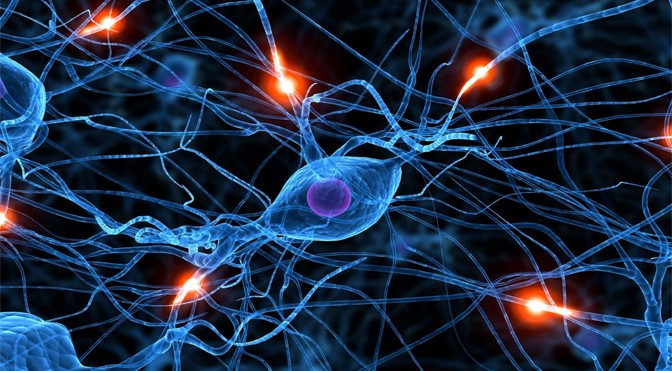
\includegraphics[width=0.75\textwidth,frame]{B1.jpeg}}
\caption*{Figure 2-1 , a Neuron in human Brain}
\label{f-1-2}
\end{figure}
%
%picture 2
\begin{figure}[h]
\centering
%\setlength{\fboxrule}{5pt}
%\fbox{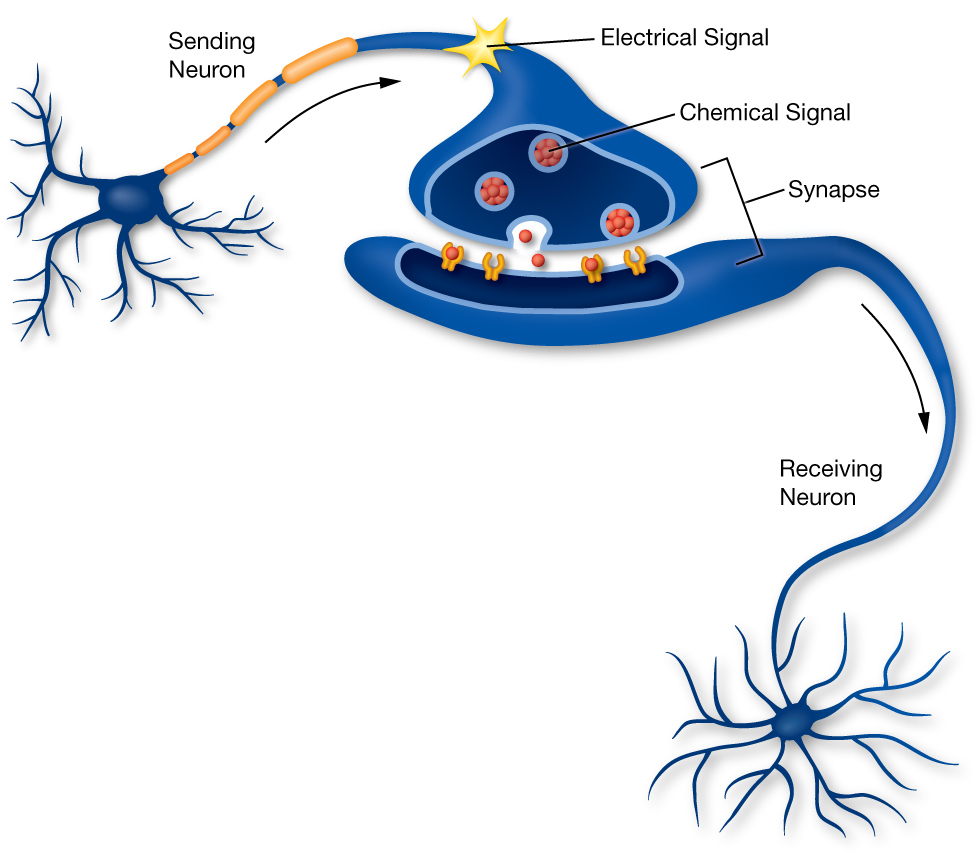
\includegraphics[width=0.75\textwidth,frame]{x.jpg}}
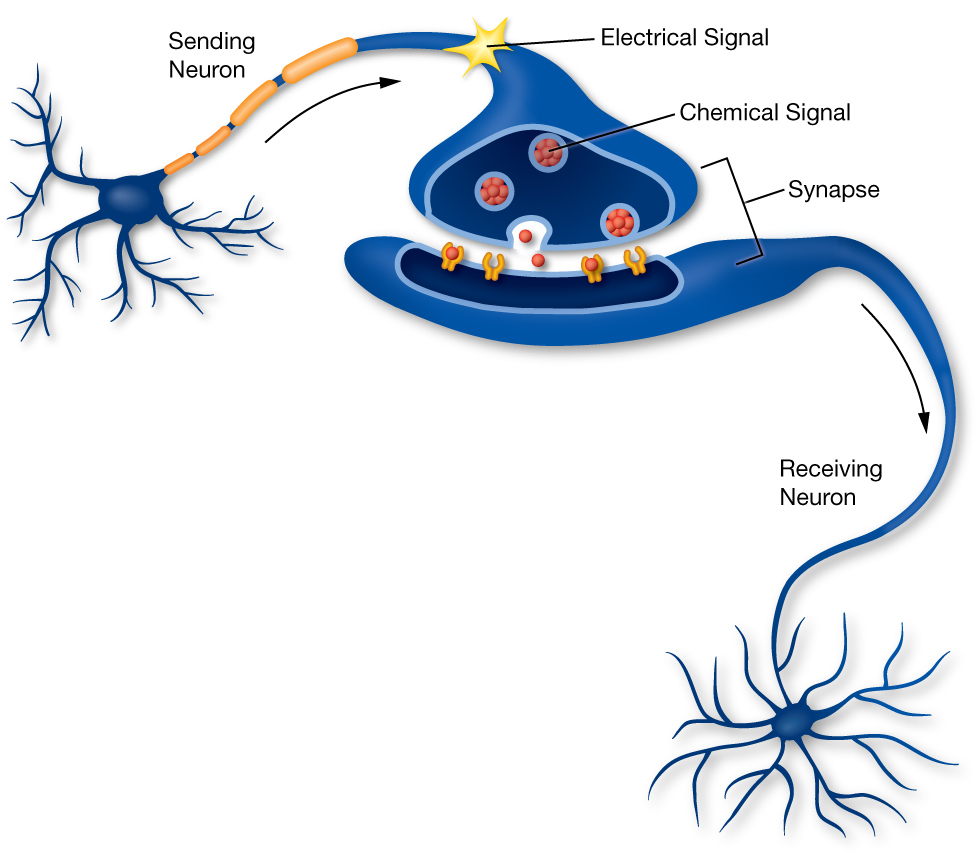
\includegraphics[width=0.75\textwidth,frame]{x.jpg}
\caption*{Figure 2-2,Figure of a Neuron Symbolyc}
\label{f-1-3}
\end{figure}

%picture 3
\begin{figure}[h]
\centering
%\setlength{\fboxrule}{5pt}
%\fbox{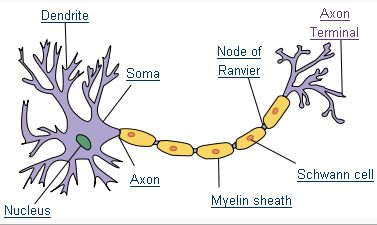
\includegraphics[width=0.75\textwidth,frame]{Neuron.jpg}}
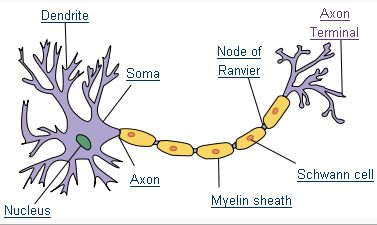
\includegraphics[width=0.75\textwidth,frame]{Neuron.jpg}
\caption*{Figure 2-3,A Closer Look At a Neuron}
\label{f-1-4}
\end{figure}


%picture 1
%\begin{center}
%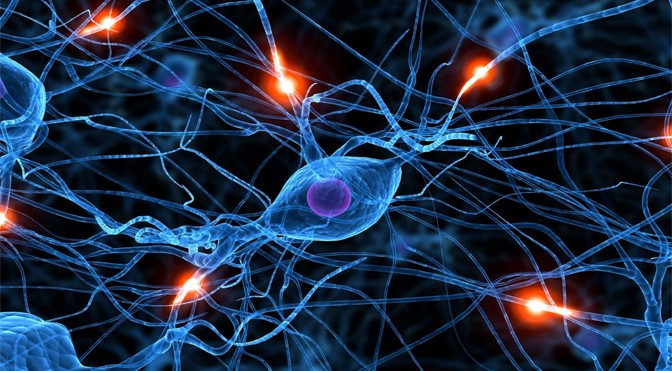
\includegraphics[width=0.75\textwidth]{B1.jpeg}
%\label{f-1-2}
%\end{center}
%

\newpage



%%%%%%%%%%%%%%%%%%%%%%%%%%%%%%%%%%%%%%%%%%%%  SECTION 2 %%%%%%%%%%%%%%%%%%%%%%%%%%%%%%%%%%%%%%%%
%%% SECTION 2
\section {What Is Machine Learning ?}
\begin{displayquote}
\textit{machine learning is the ability to learn and process for a computer due to some samples and test without implementing \textbf{extra code} for a machine.}
\[ Dr Andrew NG  -  Stanford University \]

\textit{Machine learning gives computers the ability to learn without being \textbf{explicitly }programmed.}
\[ Arthur Samuel, 1959 \]
\end{displayquote}
we can develop a machine to do a specific job with higher sensitivity and accuracy even without implementing thousand and thousands lines of code . the first idea of developing such a machine was brought up in early of 1950 ‘s . the was being ignored at first but after decades of hard work and research mankind did develop a simple easy theory to a great massive complicated technology that we are facing today in medicine , engineering and even our daily life such as smart phones and gadgets .\\
the subjects and documents of machine learning are tightly close to deep learning and artificial intelligence which is not fully covered in this article but some how pointed out in some parts .  \\

%%%%%%%%%%%%%%%%%%%%%%%%%%%%%%%%%%%%%%%%%%%%  SECTION 3 %%%%%%%%%%%%%%%%%%%%%%%%%%%%%%%%%%%%%%%%
\section  { History Of Neural Network In Machine Learning }
 
The preliminary theoretical base for contemporary neural networks was independently proposed by  \textit{Alexander Bain (1873)}   and  \textit{William James (1890)}.  In their work, both thoughts and body activity resulted from interactions among neurons within the brain.
The idea of creating a neural network was then considered by two scientists , \textit{Dr Warren Sturgis McCulloch (November 16, 1898 – September 24, 1969)}  who was an American neurophysiologist and cybernetician, known for his work on the foundation for certain brain theories and his contribution to the cybernetics movement and  \textit{Dr.Frank Rosenblatt (July 11, 1928 – July 11, 1971) }  was an American psychologist notable in the field of artificial intelligence. These two scientists created the first neural network using an electric circuit in 1943 . \\
The project of neural network simulation was not ended here . \textit{Dr. Alan Turing ( 1912 – 1954 )} ( the inventor of  \textit{Turing Machine }  and an expert in decrypting  \textit{The Enigma} during \textit{World War II} )  and \textit{Dr . John von Neumann ( 1903 – 1957 )}   were also on of the thousands of scientists who worked on neural networks .[2]


\begin{figure}[!htb]
\minipage{0.16\textwidth}
\setlength{\fboxrule}{2pt}
  \fbox{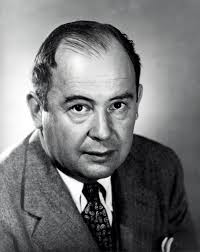
\includegraphics[width=\linewidth,frame]{s1.jpg}}
  \caption*{John von Neumann}\label{f-3-1}
\endminipage\hfill
\minipage{0.16\textwidth}
\setlength{\fboxrule}{2pt}
 \fbox{ 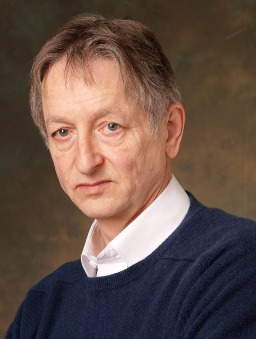
\includegraphics[width=\linewidth,frame]{s2.jpg}}
  \caption*{Frank Rosenblatt}\label{f-3-2}
\endminipage\hfill
\minipage{0.16\textwidth}%
\setlength{\fboxrule}{2pt}
  \fbox{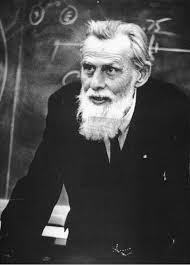
\includegraphics[width=\linewidth,frame]{s3.jpg}}
  \caption*{Warren Sturgis McCulloch}\label{f-3-3}
\endminipage\hfill
  \minipage{0.16\textwidth}%
  \setlength{\fboxrule}{2pt}
  \fbox{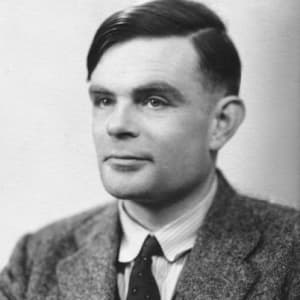
\includegraphics[width=\linewidth,frame]{s4.jpg}}
  \caption*{Alan Turing}\label{f-3-4}
\endminipage
\end{figure}

\newpage



%%%%%%%%%%%%%%%%%%%%%%%%%%%%%%%%%%%%%%%%%%%%  SECTION 4 %%%%%%%%%%%%%%%%%%%%%%%%%%%%%%%%%%%%%%%%
\section{Main Usages Of Neural Networks } 
Neural networks can be used in different fields. The tasks to which artificial neural networks are applied tend to fall within the following broad categories: \\
\begin{description}[font=$\bullet$~\normalfont\scshape\color{red!50!black}]
\item [ Function approximation], or regression analysis, including time series prediction and modeling.
\item [Classification] , including pattern and sequence recognition, novelty detection and sequential decision making.
\item [Data processing], including filtering, clustering, blind signal separation and compression.[1]

\end{description}
The usage of machine learning and neural networks are so vast and extensive these days . the most common application is automate driving which has been released and developed by big companies such as Tesla and Google . the base and fundamental of these technologies are neural networks . another applications which are quite old-fashioned but still being used is face recognition and voice recognition which has been a routine technology in modern countries like united states and Canada . \\

%%%%%%%%%%%%%%%%%%%%%%%%%%%%%%%%%%%%%%%%%%%%  SECTION 5 %%%%%%%%%%%%%%%%%%%%%%%%%%%%%%%%%%%%%
\section{ Neural Network Components }
A neural network , as it can be understood from it’s name , is a network consisted of neurons and perceptron . as we discussed in  (\hyperref [sec:1]{Section 1}) , each neuron in human brain has 3 parts . in machine learning neural network we have the same situation . each neuron has 1 \textit{''input''} layer , 1 \textit{'processing''}unit and 1\textit{''output''} layer . each neural network has at least 2 layers . the input layer and the output layer . 

%picture
\begin{figure}[h]
\centering
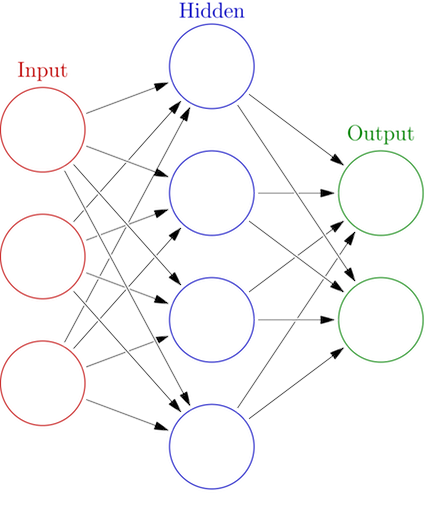
\includegraphics[width=0.3\textwidth,frame]{nn.png}
\caption*{A simple 3 layered Neural Network( figure 5-1 )}
\label{f-5-1}
\end{figure}

We can have some layers in between that are called the \textit{''hidden layers''} . we determine the number of hidden layers due to the complexity of out machine and the sensitivity of out machine . the hidden layers and their number are the base and main part of a neural network which is not totally covered in this article and would be left for the reader to search and study about them because these topics are related to advanced neural networks . \\
In a network , at each layer , one perceptron in connected to all of the neurons in the next layer and each connection has a weight which modifies how important and great each neuron can effect the input for the next layer. \\
Each neuron has also a constant amount called bias which would be added to the value before going to the next level layer . Each neuron has a number in it called “ the activation number “ which is the value of the neuron .we later on determine the output of the machine using this activation number . 
%%%%%%%%%%%%%%%%%%%%%%%%%%%%%%%%%%%%%%%%%%%%  SECTION 6 %%%%%%%%%%%%%%%%%%%%%%%%%%%%%%%%%%%%%
\section { How Does A Neural Network Work ? }
Assume that we are going to program and train a machine to recognize the hand writing of a person from another one . the application is called OCR . the problem rises when we realize that we can write a number for example “3” in many different ways . ( each person has a unique handwriting which means we have a unique pattern for each human to write a single number such as 3 )\\
If we give a sheet of paper to a person to write a number and take a picture of that sheet of paper and putting it in a 28x28 pixel picture , then we are going to have 784 pixels totally . if we assume each pixel as a neuron , then we are going to have a neural network with 784 neurons as it’s input and 10 neurons as it’s output referencing a number between 0 to 9 . \\
Let me explain the main idea by using an example. Assume we have number “9” . if we break number 9 into two fractions which make the figure of nine we can obviously see a circle and a bended line ( O +  I ) and if we break each of two component s into multiple fraction parts as the figure shows .we can see that obviously we have 2 layers that help us create number nine . now if our machine becomes able to create a number step by step ( by creating each fractional part of a number in each layer ) then our machine would finally be able to recognize any number given . \\
You can see a simple and basic routine through the pictures shown below .[3] \\




%picture
\begin{figure}[H]
\centering
\setlength{\fboxrule}{5pt}
\fbox{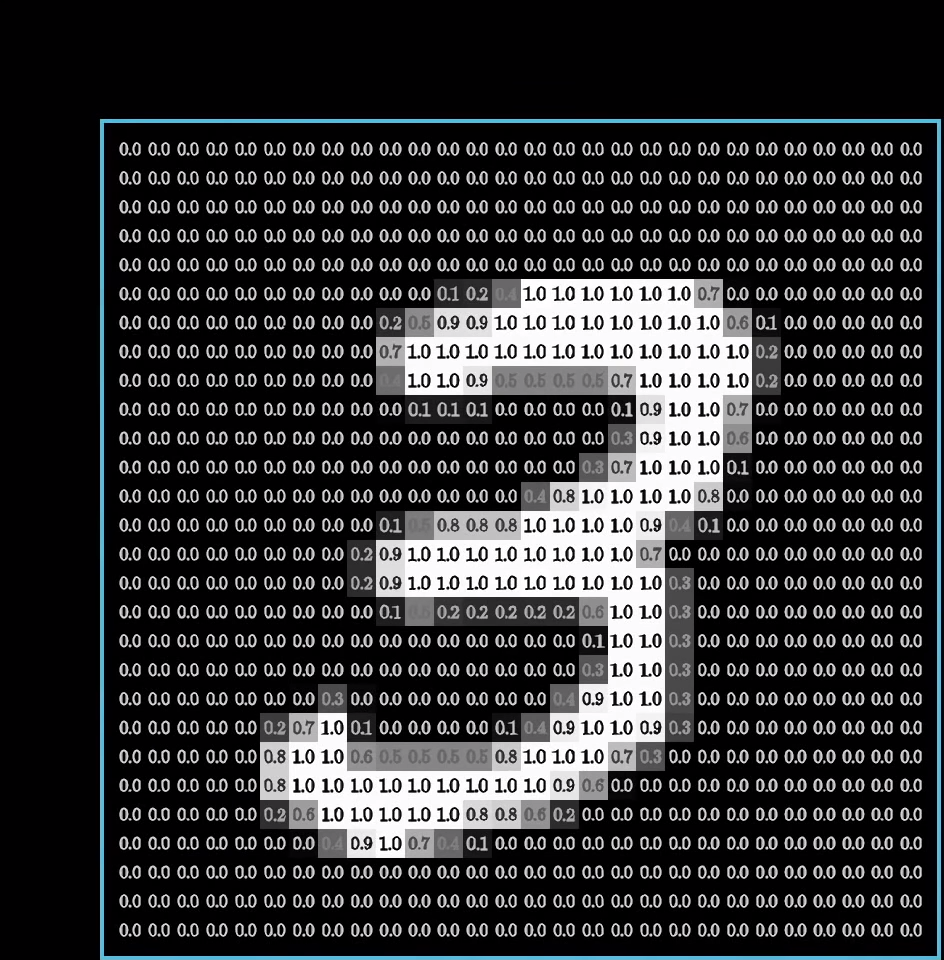
\includegraphics[width=0.4\textwidth,frame]{1.png}}
\caption*{Figure 7-1}
\label{f-6-1}
\end{figure}


%picture
\begin{figure}[H]
\centering
\setlength{\fboxrule}{5pt}
\fbox{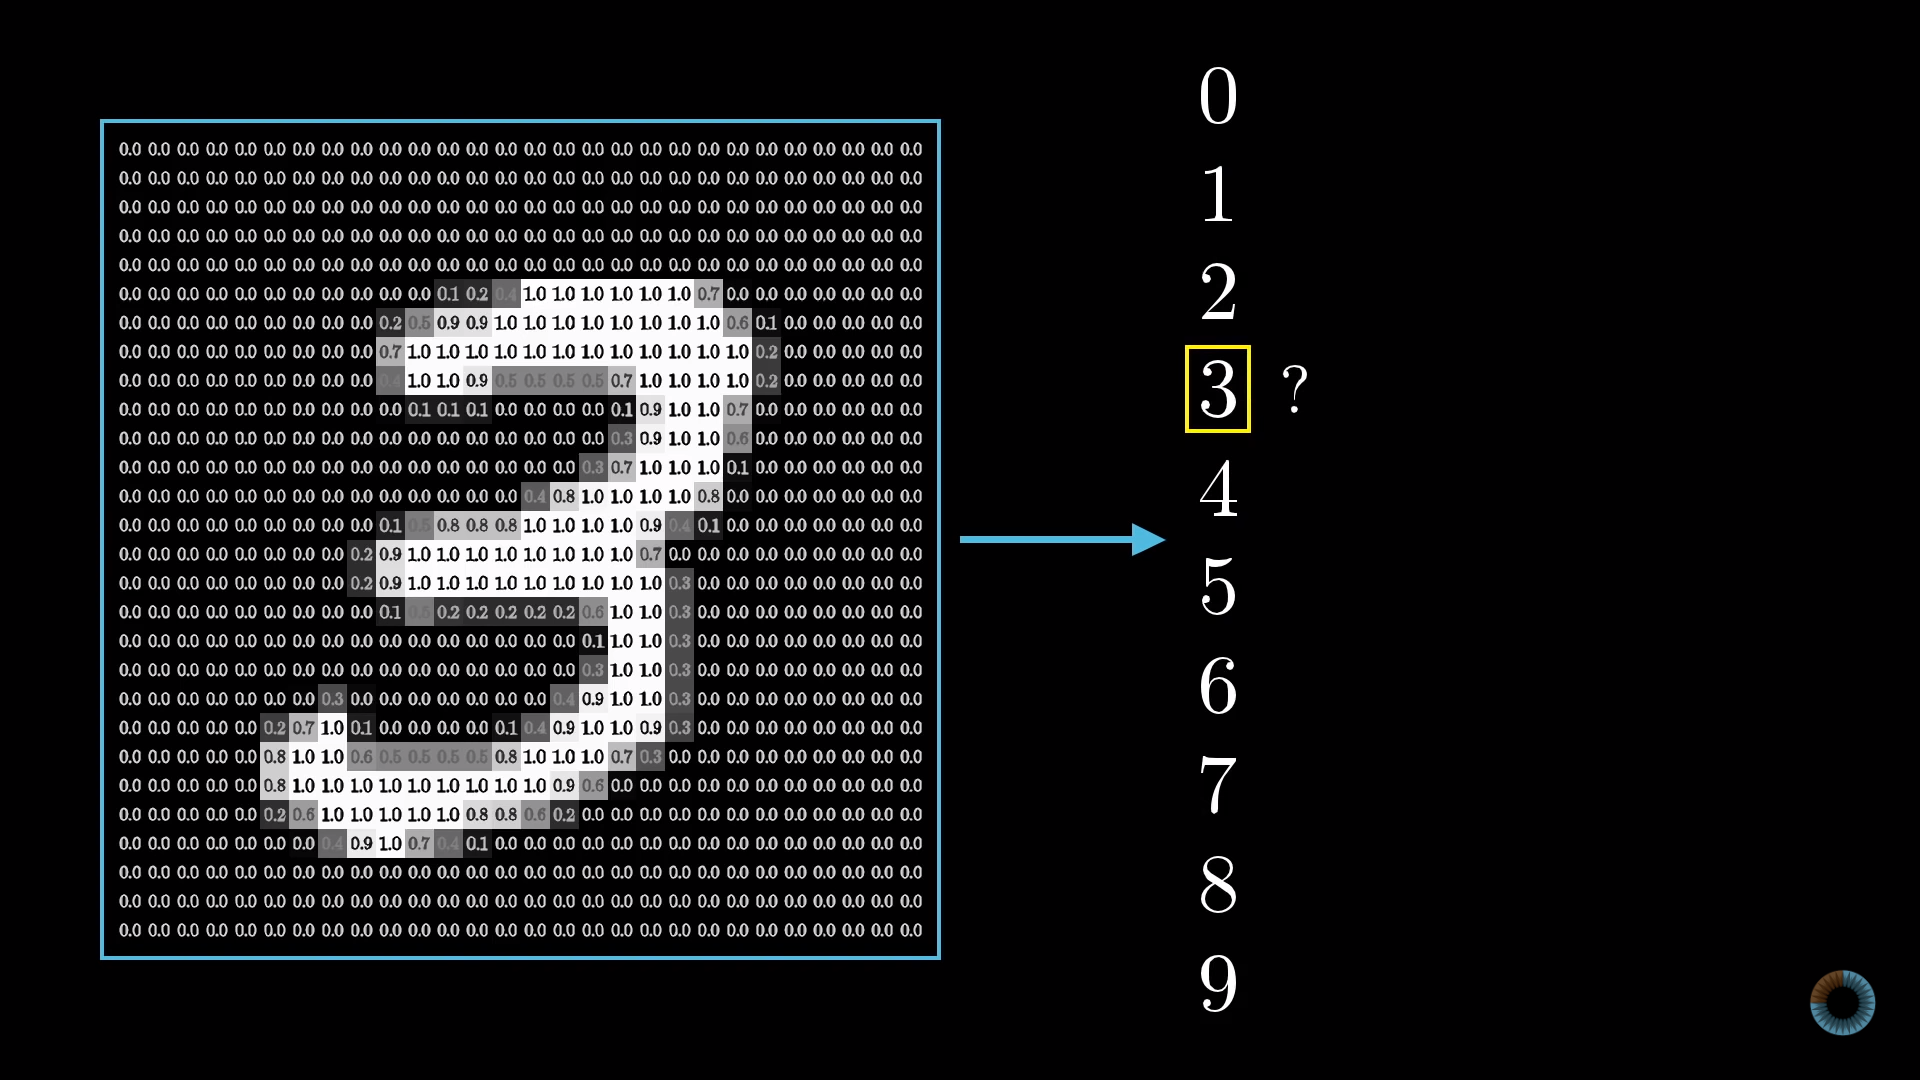
\includegraphics[width=0.9\textwidth,frame]{2.png}}
\caption*{Figure 7-2}
\label{f-6-2}
\end{figure}


%picture
\begin{figure}[H]
\centering
\setlength{\fboxrule}{5pt}
\fbox{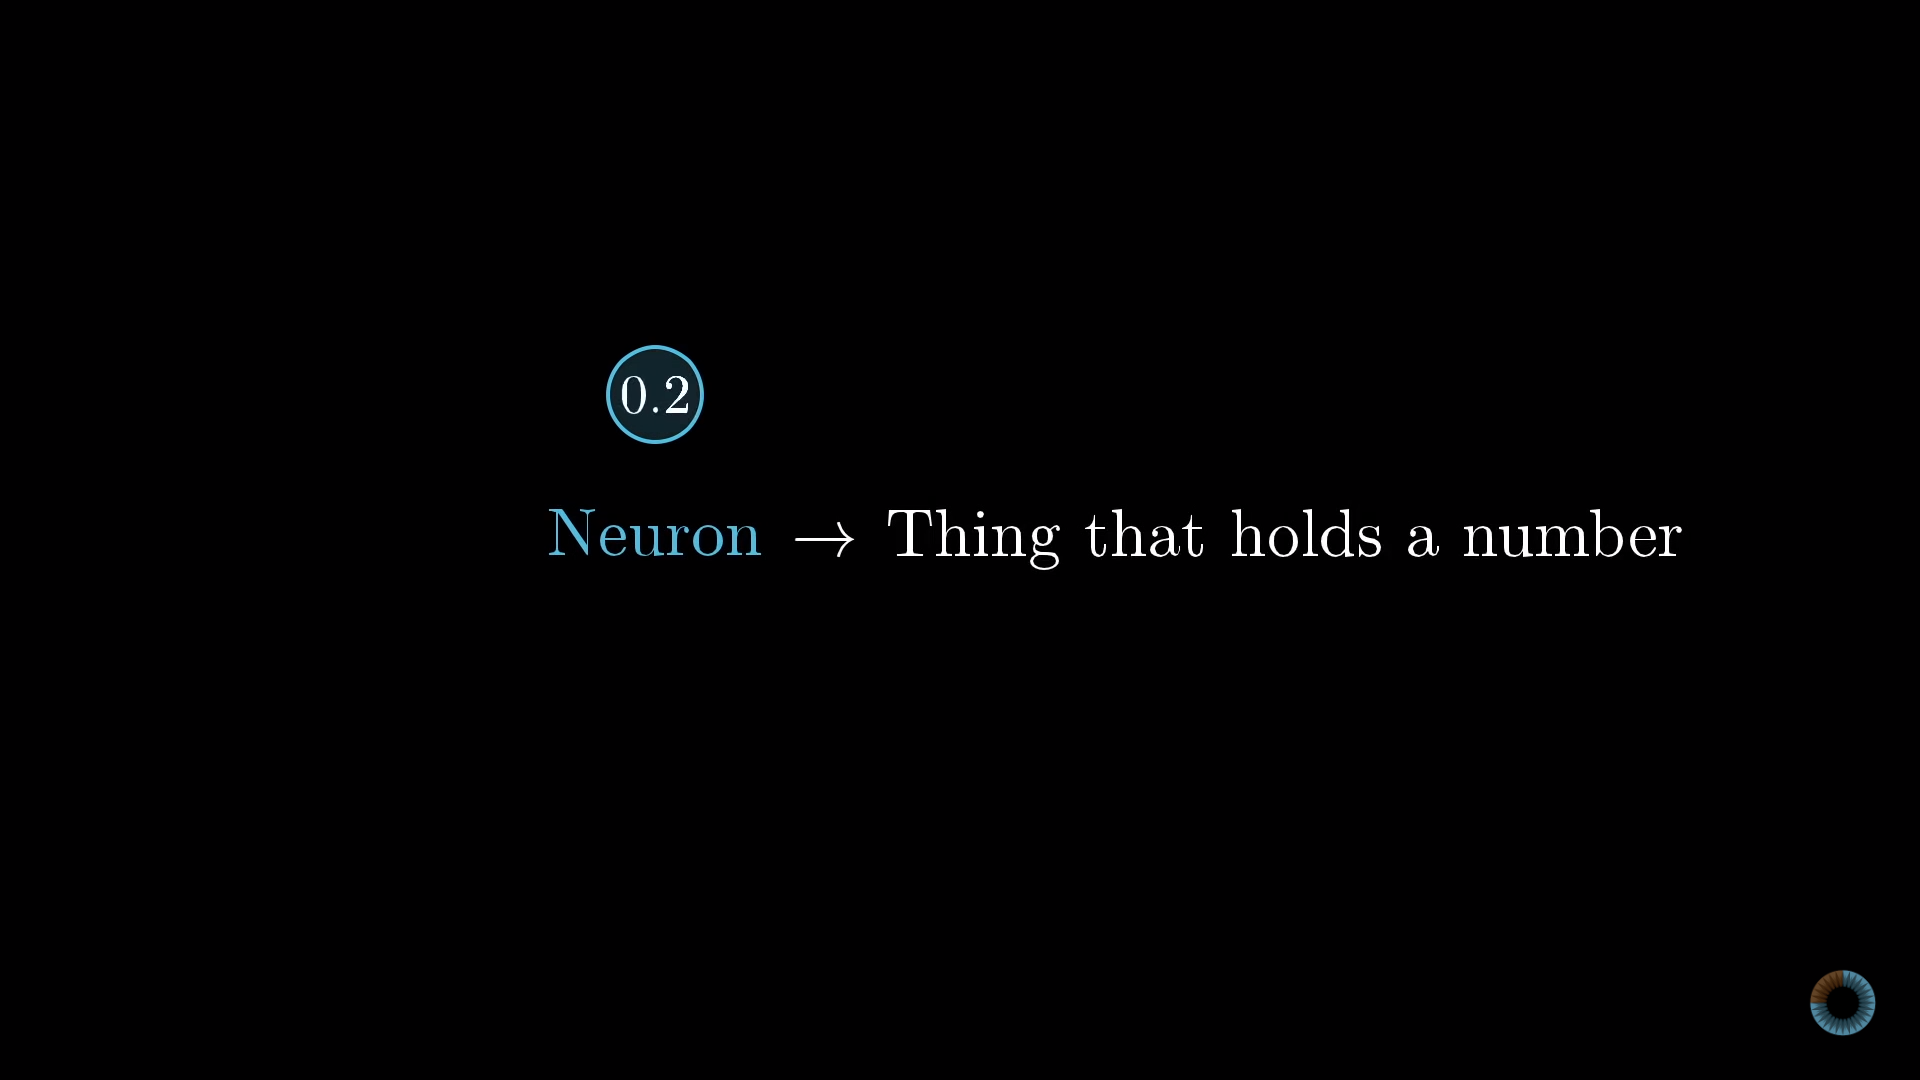
\includegraphics[width=0.9\textwidth,frame]{3.png}}
\caption*{Figure 7-3}
\label{f-6-3}
\end{figure}


%picture
\begin{figure}[H]
\centering
\setlength{\fboxrule}{5pt}
\fbox{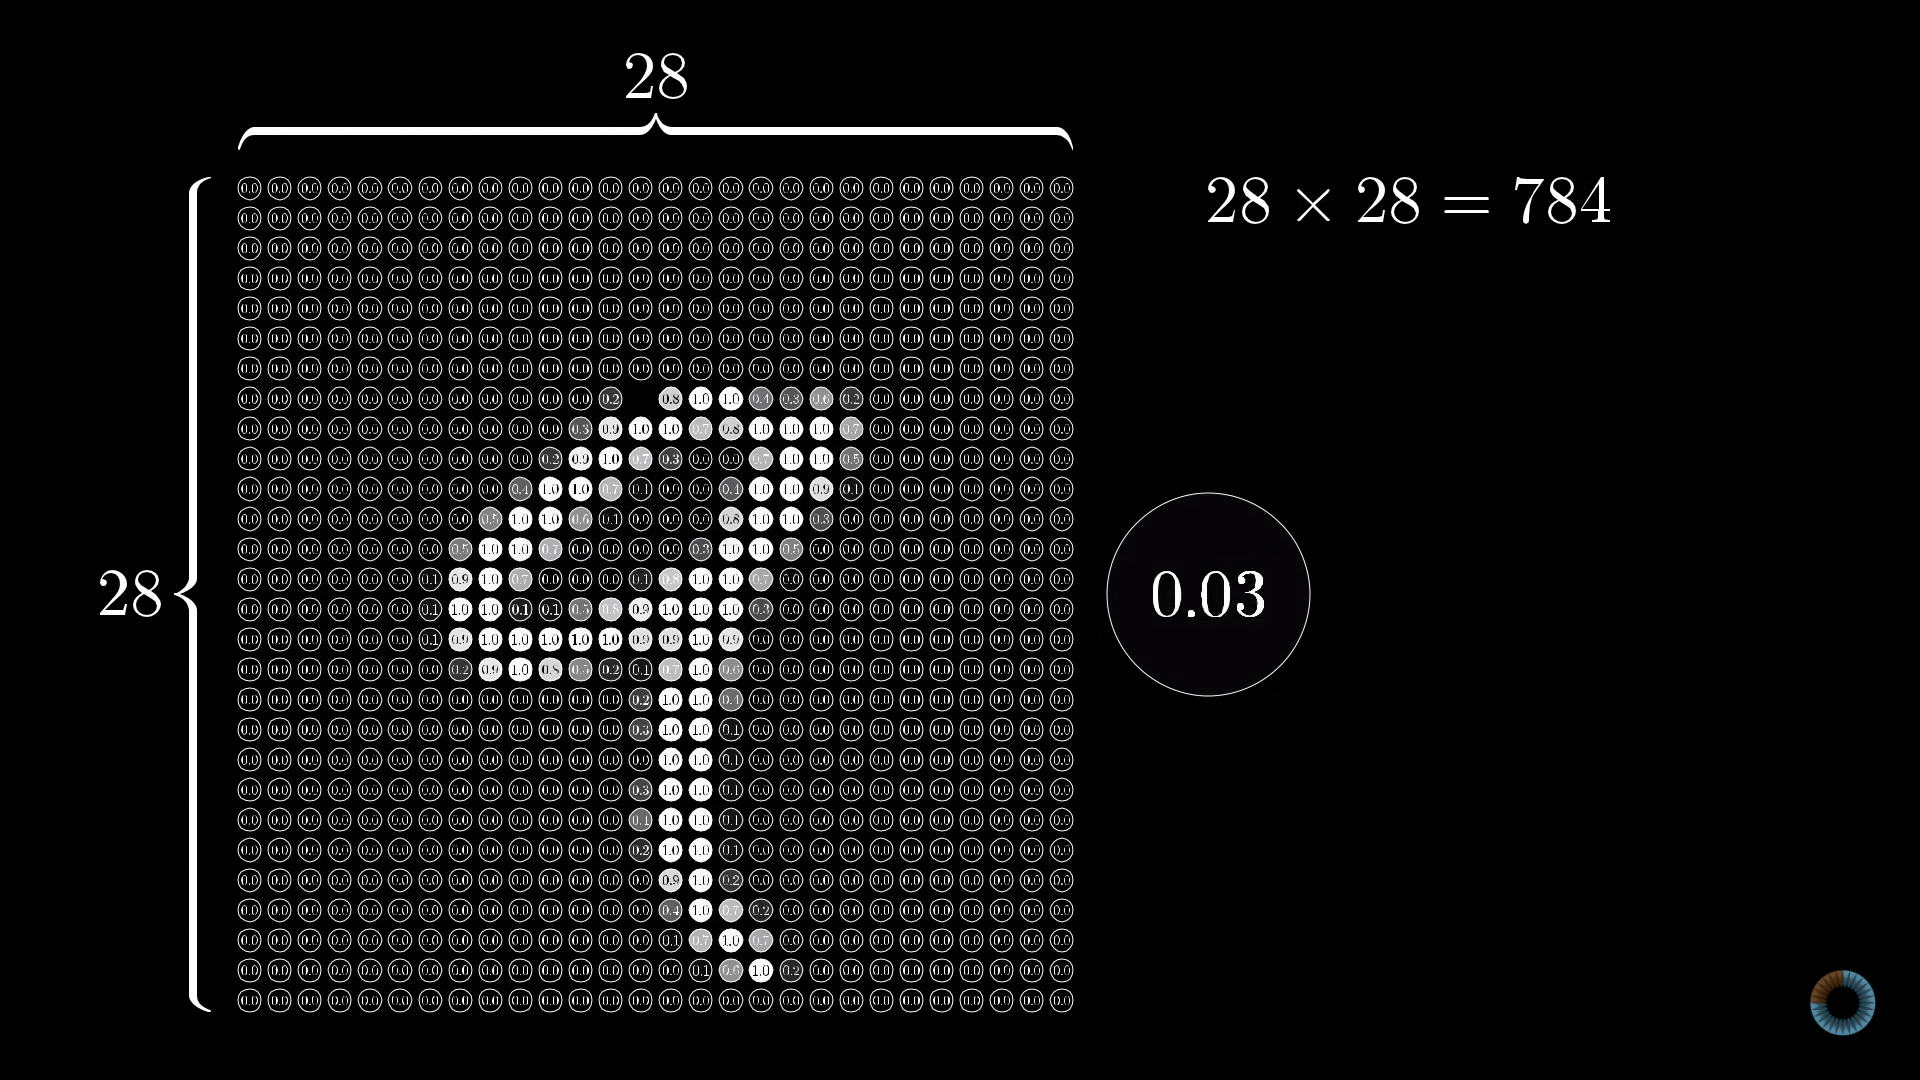
\includegraphics[width=0.9\textwidth,frame]{4.png}}
\caption*{Figure 7-4}
\label{f-6-4}
\end{figure}


%picture
\begin{figure}[H]
\centering
\setlength{\fboxrule}{5pt}
\fbox{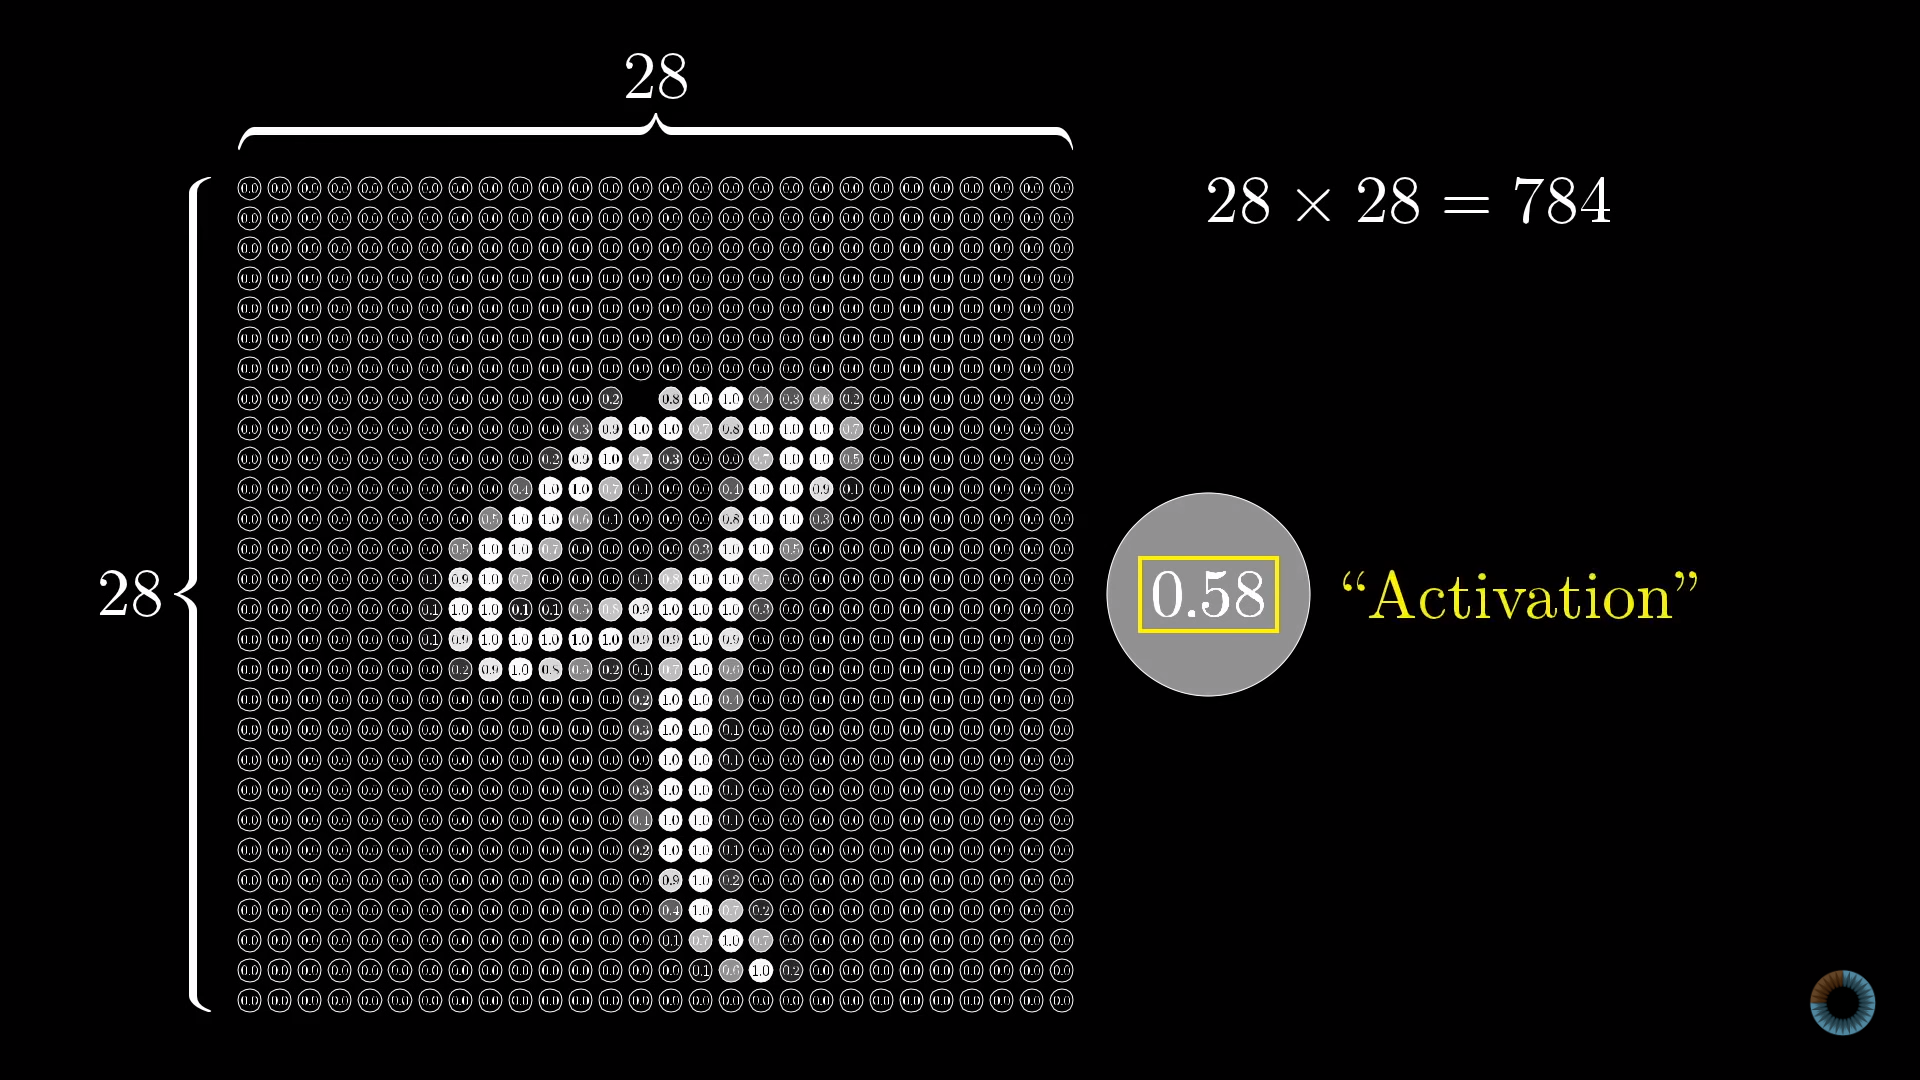
\includegraphics[width=0.9\textwidth,frame]{5.png}}
\caption*{Figure 7-5}
\label{f-6-5}
\end{figure}


%picture
\begin{figure}[H]
\centering
\setlength{\fboxrule}{5pt}
\fbox{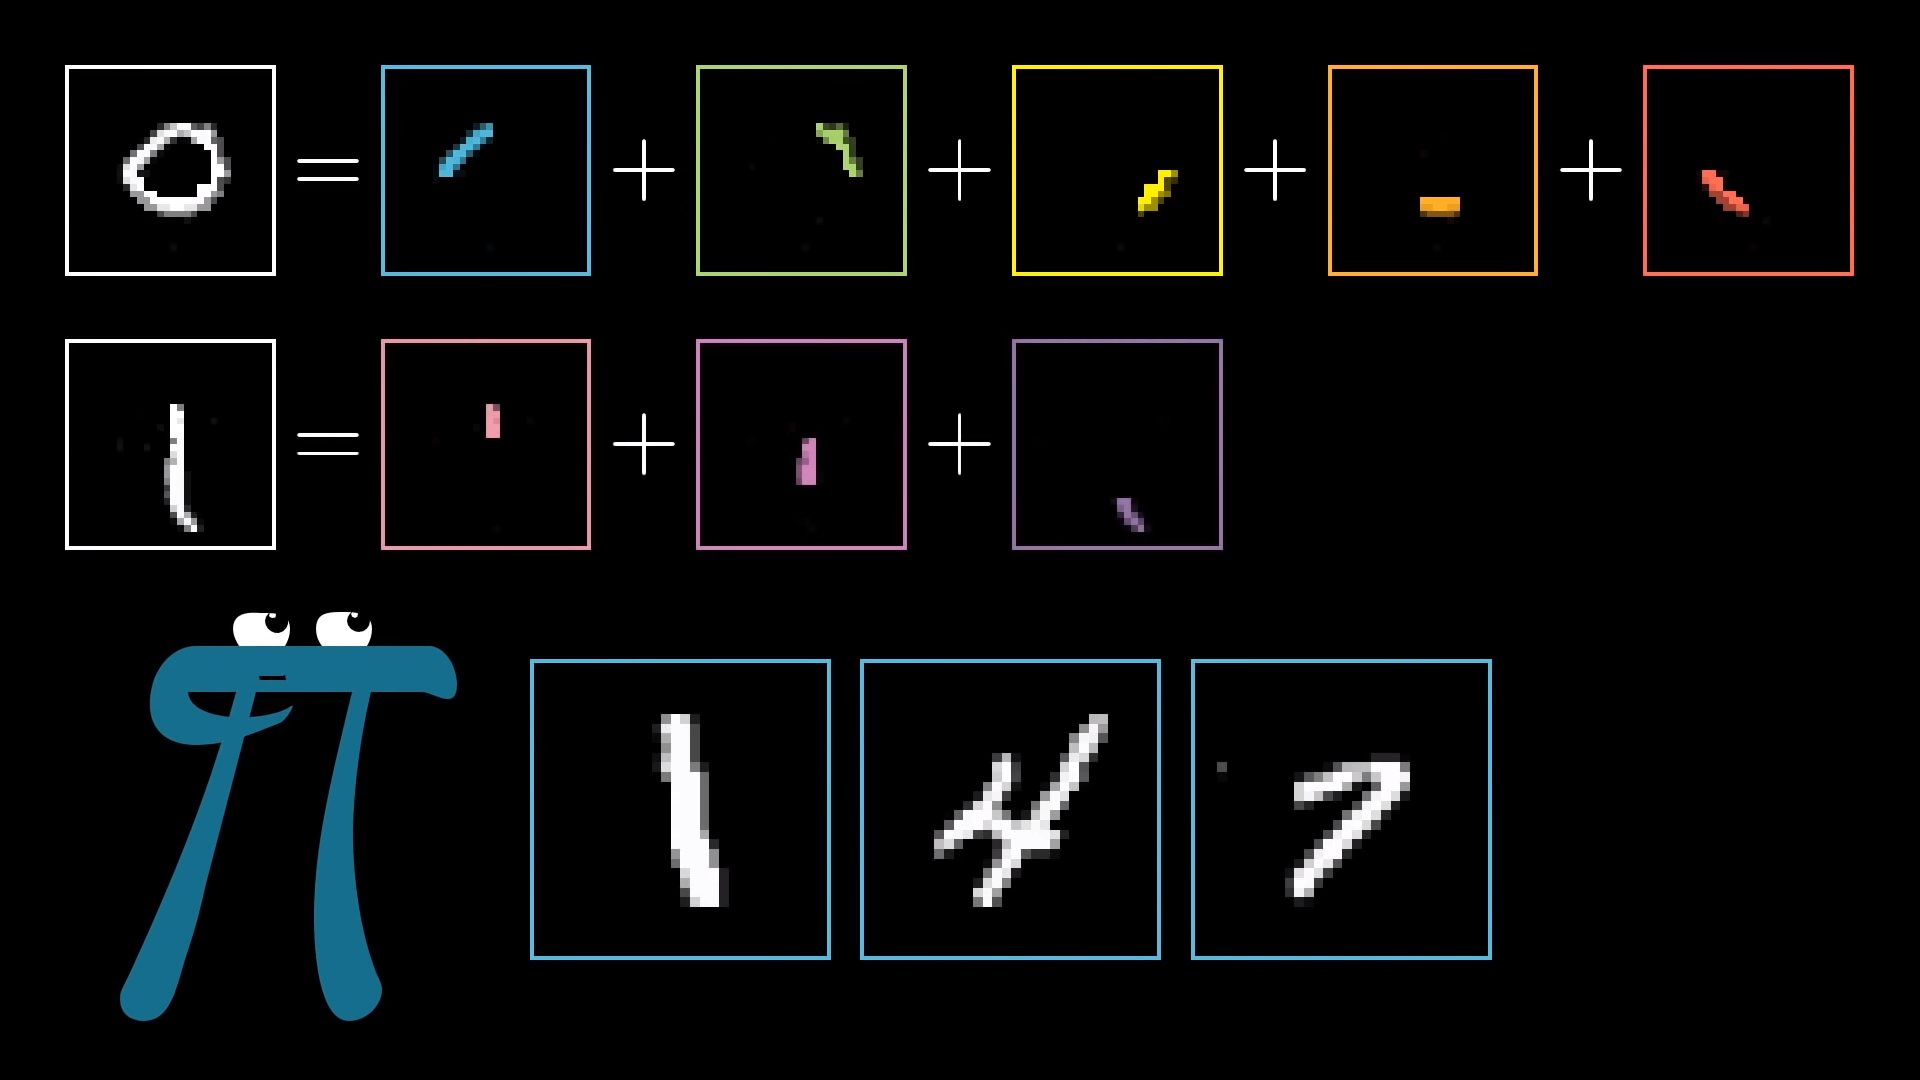
\includegraphics[width=0.9\textwidth,frame]{6.png}}
\caption*{Figure 7-6}
\label{f-6-6}
\end{figure}


%picture
\begin{figure}[H]
\centering
\setlength{\fboxrule}{5pt}
\fbox{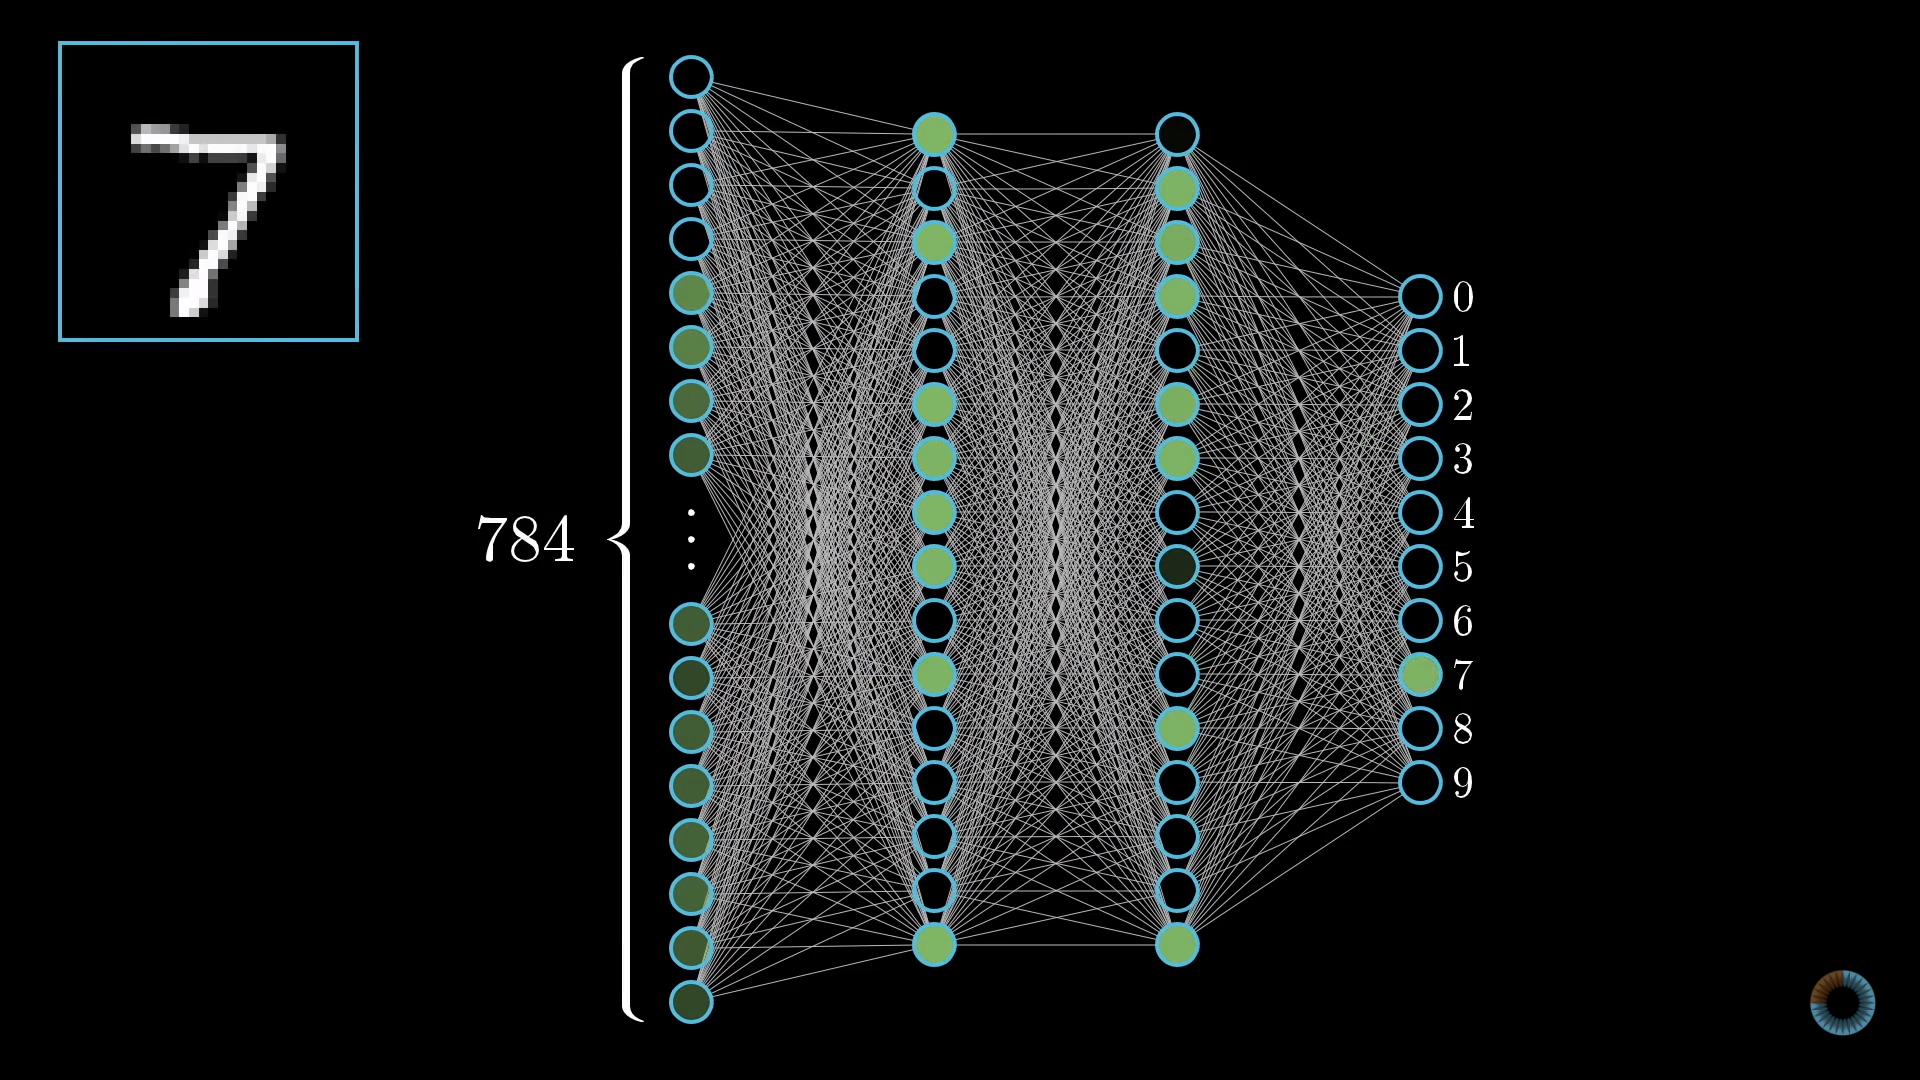
\includegraphics[width=0.9\textwidth,frame]{7.png}}
\caption*{Figure 7-7}
\label{f-6-7}
\end{figure}


%picture
\begin{figure}[H]
\centering
\setlength{\fboxrule}{5pt}
\fbox{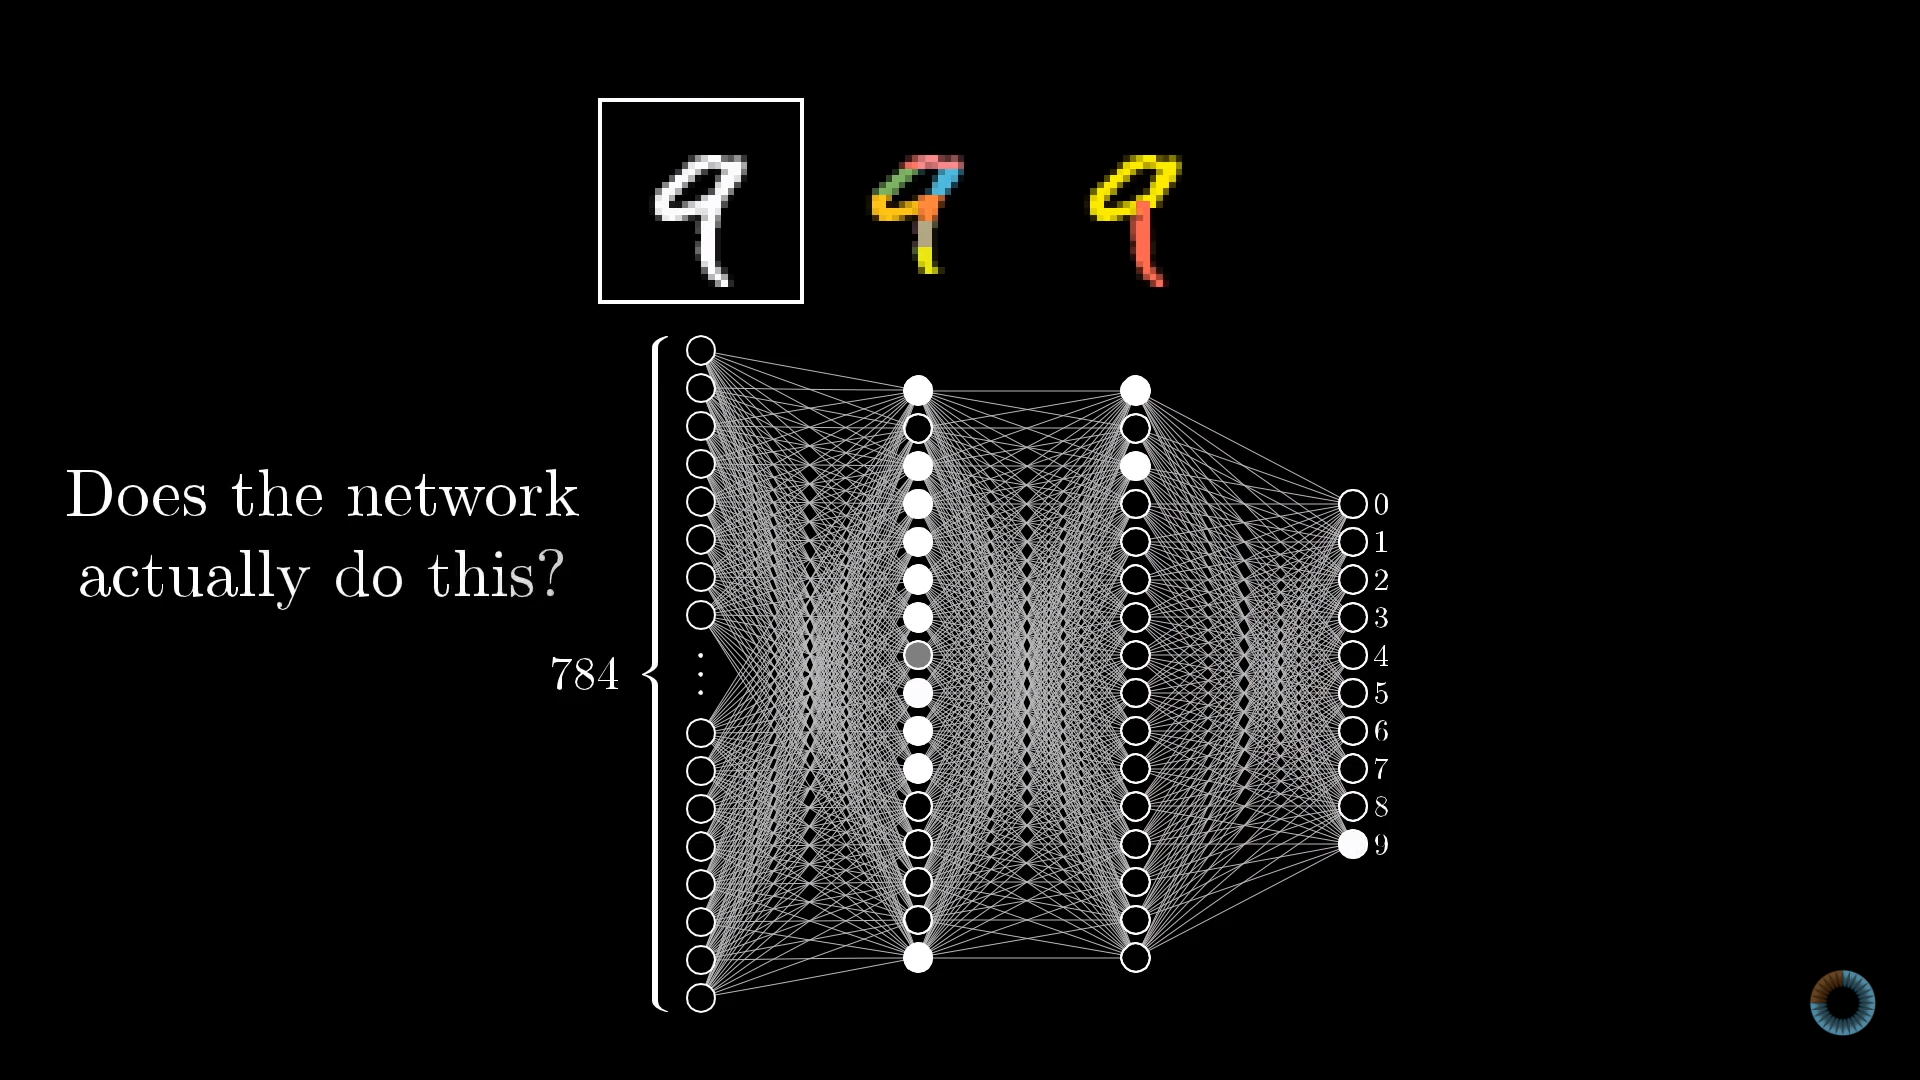
\includegraphics[width=0.9\textwidth,frame]{8.png}}
\caption*{Figure 7-8}
\label{f-6-8}
\end{figure}


%picture
\begin{figure}[H]
\centering
\setlength{\fboxrule}{5pt}
\fbox{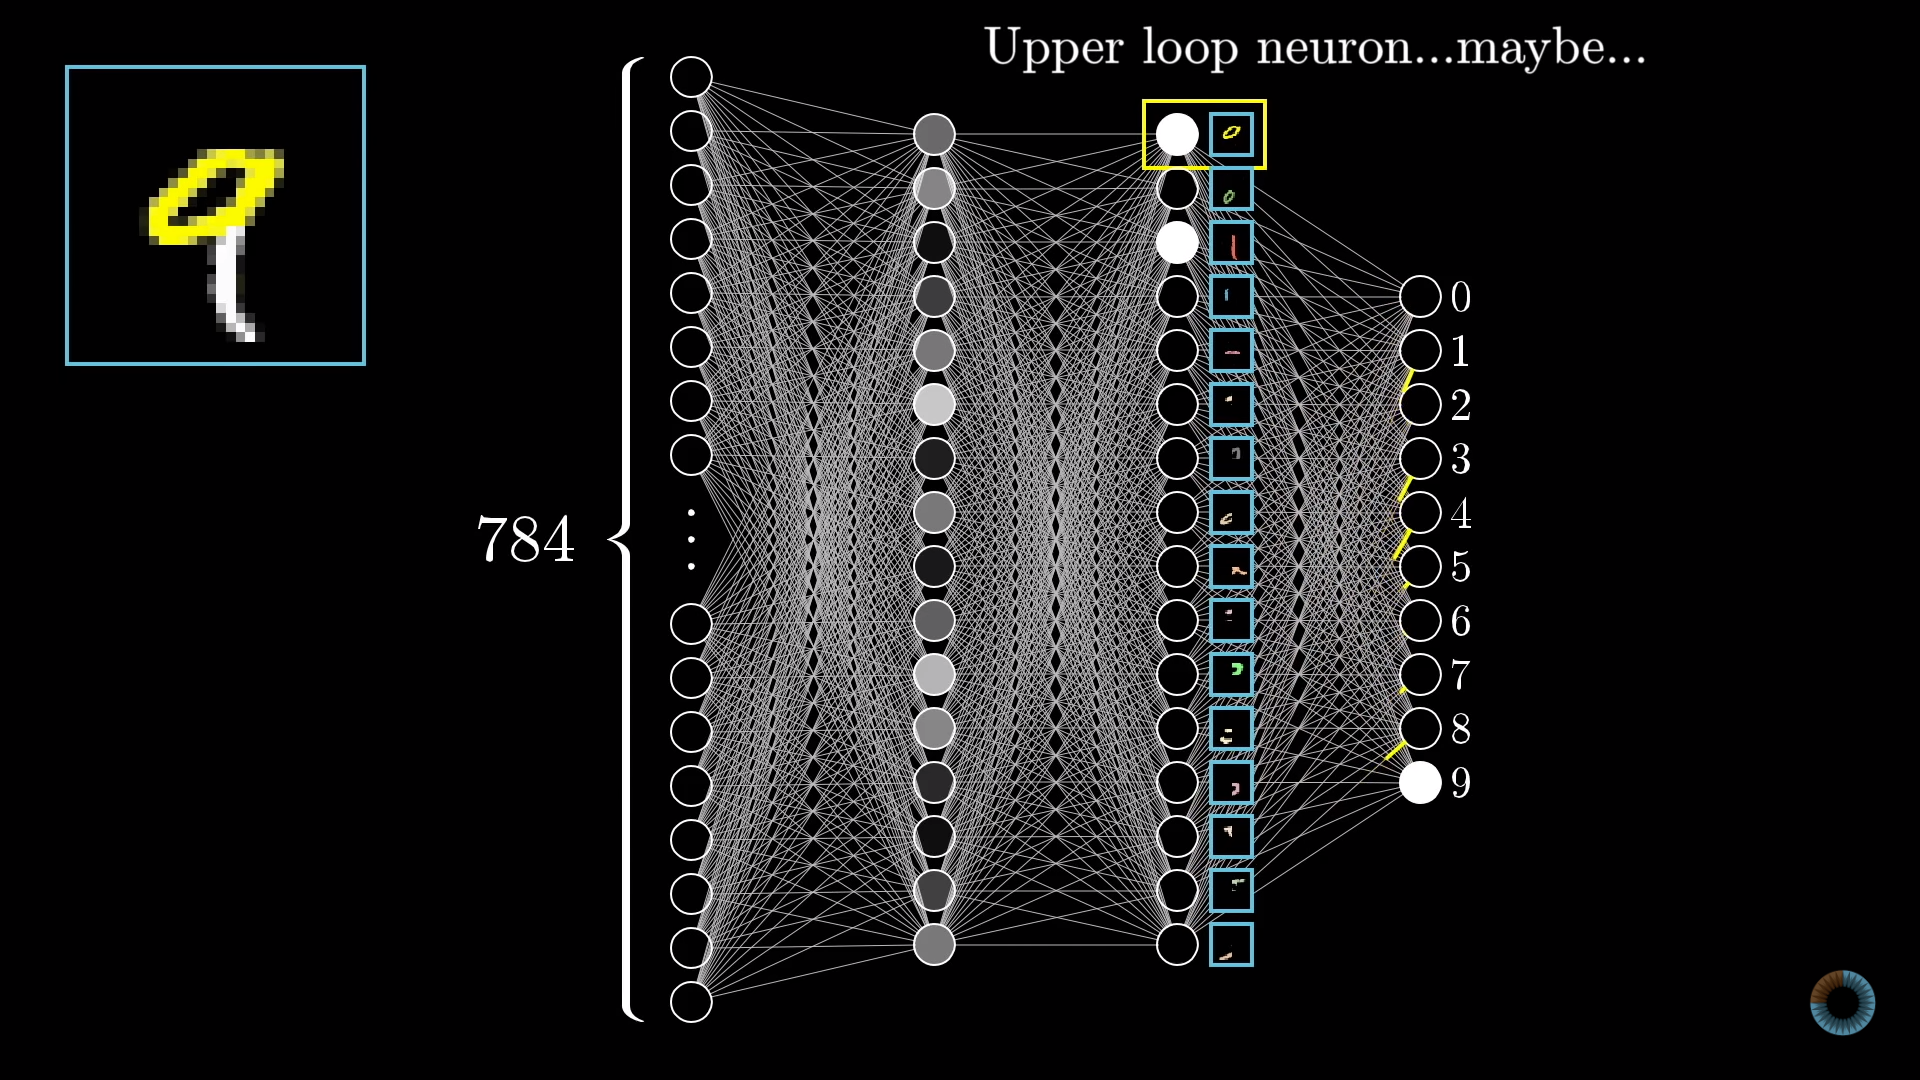
\includegraphics[width=0.9\textwidth,frame]{9.png}}
\caption*{Figure 7-9}
\label{f-6-9}
\end{figure}





In  \hyperref [f-5-1]{Figure 5-1}  and \hyperref [f-6-9]{Figure 7-9} you can see that each node in our graph has a connection to the other node in the next layer . each connection has a weight as we mentioned before . in a simple network with 4 layers and each layer having\textit{ 784 , 16 ,16 , 9 }nodes , we will have 1,806,336 weights totally to be numbered and set . this huge amount of processing would be accomplished by huge amount of datasets . we have to train our machine by giving it a lot of entries with their correct answers . how do we train it ? simple . we assume that we are going to recognize number ''9'' . we give the machine multiple entries that finally get to number ''9'' . at each layer we have to reach a certain answer so we have to set the weights of the connections some how to get us to the wanted answer . we call this method propagation . if we start the \textbf{\textit{propagation} } from the output layer and finally reach the input layer it would be called \textbf{\textit{backpropagation} }  and if we start from initial layer and reach the output layer we call it \textbf{\textit{forward propagation} } .in calculating the activation number of each node we might get to numbers too big or too small . in order to limit the activations between a upper bound and a lower bound we use the sigmoid function which constraints the activations between 0 to 1 . we have some other methods to reach the most optimized weights and biases for each node . one of them is Gradient descent which is very useful and popular In different branches of deep learning . these subjects are not covered in this article and they would be left to the reader . [1]

%%%%%%%%%%%%%%%%%%%%%%%%%%%%%%%%%%%%%%%%%%%%  Summary %%%%%%%%%%%%%%%%%%%%%%%%%%%%%%%%%%%%%
\section { Keywords } 
Machine learning , Neural Networks ,Perceptron , Node , Weight , Bias , Networks ,   Sigmoid Function 

%%%%%%%%%%%%%%%%%%%%%%%%%%%%%%%%%%%%%%%%%%%%  Keywords %%%%%%%%%%%%%%%%%%%%%%%%%%%%%%%%%%%%%

\section{Summary}
A neural network is a network or circuit of neurons, or in a modern sense, an artificial neural network, composed of artificial neurons or nodes.[1] Thus a neural network is either a biological neural network, made up of real biological neurons, or an artificial neural network, for solving Artificial Intelligence (AI) problems. The connections of the biological neuron are modeled as weights. A positive weight reflects an excitatory connection, while negative values mean inhibitory connections. All inputs are modified by a weight and summed. This activity is referred as a linear combination. Finally, an activation function controls the amplitude of the output. These artificial networks may be used for predictive modeling, adaptive control and applications where they can be trained via a dataset. Self-learning resulting from experience can occur within networks, which can derive conclusions from a complex and seemingly unrelated set of information.
\newpage
%----------------------------------------------------------------------------------------
%	BIBLIOGRAPHY
%----------------------------------------------------------------------------------------

\begin{thebibliography}{9}
\bibitem{Machine Learning and It's Applications} 
Dr. Andrew NG, University Of Stanford. 

 
\bibitem{Neural Networks and Machine Learning} 
Wikipedia.

 
\bibitem{Neural Networks and Depp Learning}
3Blue1Brown Course 

\end{thebibliography}











\LaTeX

\end{document}